\documentclass[10pt]{article}
\usepackage[polish]{babel}
\usepackage[utf8]{inputenc}
\usepackage[T1]{fontenc}
\usepackage{graphicx}
\usepackage[export]{adjustbox}
\graphicspath{ {./images/} }
\usepackage{amsmath}
\usepackage{amsfonts}
\usepackage{amssymb}
\usepackage[version=4]{mhchem}
\usepackage{stmaryrd}

\title{GIMNAZJUM }

\author{}
\date{}


\begin{document}
\maketitle
\begin{center}
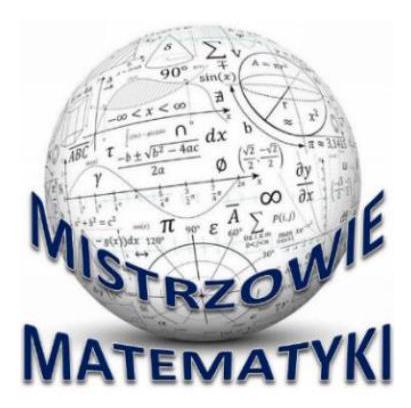
\includegraphics[max width=\textwidth]{2024_11_21_e3816fc2ecd6c27612f5g-1}
\end{center}

\begin{enumerate}
  \item Czy wierzchołki 20-kąta foremnego można tak ponumerować liczbami 1,2,...,20, aby użyć wszystkich tych liczb oraz aby dla każdych czterech kolejnych wierzchołków suma ich numerów była mniejsza od 43? Odpowiedź uzasadnij.
  \item Dziewięciokąt foremny podzielono jego przekątnymi na trójkąty i co drugi z nich pomalowano na niebiesko. Która część wielokąta ma większe pole: niebieska czy biała?\\
Odpowiedź uzasadnij.\\
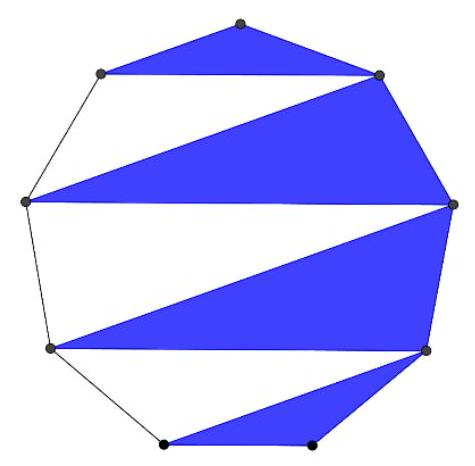
\includegraphics[max width=\textwidth, center]{2024_11_21_e3816fc2ecd6c27612f5g-1(1)}
  \item Oblicz wartość ułamka \(\frac{36 \cdot 18^{n}-8 \cdot 2^{n-4} \cdot 9^{n}-3^{n+1} \cdot 6^{n+1}}{18^{n-1}}\), gdzie \(n\) jest liczbą naturalną.
\end{enumerate}

\section*{LICEUM}
\begin{enumerate}
  \item Oblicz \(\sqrt{\underbrace{44 \ldots 4}_{2 n}+\underbrace{11 \ldots 1}_{n+1}-\underbrace{66 \ldots 6}_{n}}\)
  \item Udowodnij, że istnieje nieskończenie wiele trójek ( \(a, b, c\) ) dodatnich liczb całkowitych spełniających równość.
\end{enumerate}

\[
a^{3}+3 b^{6}=c^{2}
\]

\begin{enumerate}
  \setcounter{enumi}{2}
  \item Dany jest okrąg \(o\) i jego cięciwa \(A B\) niebędąca średnicą. Na okręgu \(o\) wybieramy punkt \(P\), różny od punktów \(A\) i \(B\). Punkty \(Q\) i \(R\) leżą odpowiednio na prostych \(P A\) i \(P B\), przy czym \(Q P=Q B\) oraz \(R P=R A\). Punkt \(M\) jest środkiem odcinka \(Q R\). Wykazać, że wszystkie uzyskane w ten sposób proste \(P M\) (odpowiadające różnym położeniom punktu \(P\) na okręgu o) mają punkt wspólny.
\end{enumerate}

\end{document}